\documentclass[9pt,twocolumn,twoside,]{pnas-new}

% Use the lineno option to display guide line numbers if required.
% Note that the use of elements such as single-column equations
% may affect the guide line number alignment.


\usepackage[T1]{fontenc}
\usepackage[utf8]{inputenc}

% tightlist command for lists without linebreak
\providecommand{\tightlist}{%
  \setlength{\itemsep}{0pt}\setlength{\parskip}{0pt}}


% Pandoc citation processing
\newlength{\cslhangindent}
\setlength{\cslhangindent}{1.5em}
\newlength{\csllabelwidth}
\setlength{\csllabelwidth}{3em}
\newlength{\cslentryspacingunit} % times entry-spacing
\setlength{\cslentryspacingunit}{\parskip}
% for Pandoc 2.8 to 2.10.1
\newenvironment{cslreferences}%
  {}%
  {\par}
% For Pandoc 2.11+
\newenvironment{CSLReferences}[2] % #1 hanging-ident, #2 entry spacing
 {% don't indent paragraphs
  \setlength{\parindent}{0pt}
  % turn on hanging indent if param 1 is 1
  \ifodd #1
  \let\oldpar\par
  \def\par{\hangindent=\cslhangindent\oldpar}
  \fi
  % set entry spacing
  \setlength{\parskip}{#2\cslentryspacingunit}
 }%
 {}
\usepackage{calc}
\newcommand{\CSLBlock}[1]{#1\hfill\break}
\newcommand{\CSLLeftMargin}[1]{\parbox[t]{\csllabelwidth}{#1}}
\newcommand{\CSLRightInline}[1]{\parbox[t]{\linewidth - \csllabelwidth}{#1}\break}
\newcommand{\CSLIndent}[1]{\hspace{\cslhangindent}#1}


\templatetype{pnasresearcharticle}  % Choose template

\title{Les standards de reproductibilité, un principe important en
recherche.}

\author[a]{Laura Béland}

  \affil[a]{Université de Sherbrooke, Départment de biologie, 2500
Boulevard de l'Université, Sherbrooke, Québec, J1K 2R1}


% Please give the surname of the lead author for the running footer
\leadauthor{}

% Please add here a significance statement to explain the relevance of your work
\significancestatement{}


\authorcontributions{}



\correspondingauthor{\textsuperscript{} }

% Keywords are not mandatory, but authors are strongly encouraged to provide them. If provided, please include two to five keywords, separated by the pipe symbol, e.g:
 \keywords{  logiciels |  prise de
données |  protocole |  reproductibilité |  transparence  } 

\begin{abstract}
Avec le taux de publication dans des sites de prépublication, les
standards de reproductibilité sont de plus en plus importants pour la
science, car il est de plus en plus difficile d'obtenir une science
juste. Il est possible d'avoir des bons standards en pennant soins de
bien gérer nos données, d'utiliser des logiciels qui permettent une
meilleure analyse des données en plus de détecter des erreurs
potentielles qui affecteraient la reproductibilité et d'offrir une
transparence au niveau des données et de l'analyse des études. Ainsi,
avec ce type de standards, la science pourra avancer plus rapidement.
\end{abstract}

\dates{This manuscript was compiled on \today}
\doi{\url{www.pnas.org/cgi/doi/10.1073/pnas.XXXXXXXXXX}}

\begin{document}

% Optional adjustment to line up main text (after abstract) of first page with line numbers, when using both lineno and twocolumn options.
% You should only change this length when you've finalised the article contents.
\verticaladjustment{-2pt}



\maketitle
\thispagestyle{firststyle}
\ifthenelse{\boolean{shortarticle}}{\ifthenelse{\boolean{singlecolumn}}{\abscontentformatted}{\abscontent}}{}

% If your first paragraph (i.e. with the \dropcap) contains a list environment (quote, quotation, theorem, definition, enumerate, itemize...), the line after the list may have some extra indentation. If this is the case, add \parshape=0 to the end of the list environment.

\acknow{}

\hypertarget{introduction}{%
\section{Introduction}\label{introduction}}

Je veux juste que sa fonctionne Depuis la pandémie, la quantité
d'articles scientifiques publiée sur des sites de prépublication à
énormément augmenté. Cet accès facile à la publication sans délais
importants et sans révisions par les paires est intéressant pour les
chercheurs qui veulent faire connaître leurs recherches et cherchent la
reconnaissance dans leur domaine. Cependant, un article publié dans de
tels sites n'est pas révisé et peut contenir plusieurs erreurs qui,
normalement, auraient pu être détectées avec la publication par des
réviseurs. De plus, le plus grand problème est le faible taux de
réplication de ses articles. Normalement, un journal scientifique va
effectuer une révision d'un article reçue pour, ainsi, minimiser les
erreurs potentielles. Cependant, même après une révision, la
reproductibilité des expérimentations scientifiques est quelque chose de
difficile à atteindre. La majorité des chercheurs, soit près de 70\%,
affirment n'ayant pas réussi à reproduire l'expérience d'un autre
chercheur ((1)). Ainsi, la reproductibilité des résultats obtenus dans
ses articles peut être difficile.

Le but de cet essai est de permettre aux chercheurs de comprendre
l'importance des principes de standards de reproduction, en mettant de
l'avant des stratégies tel que la prise de données, l'utilisation de
divers logiciels, ainsi que la transparence.

\hypertarget{mise-en-contexte}{%
\section{Mise en contexte}\label{mise-en-contexte}}

Étant donnée la grande augmentation de rapport de recherche mis à la
disposition du public sur les sites de prépublication, la
reproductibilité est de plus en importante. Elle permet de s'assurer
d'un minimum d'erreur dans les données d'une analyse, ainsi que
d'assurer la fiabilité des résultats obtenus et que l'analyse est juste.
Comme les résultats des articles prépubliés pourraient faire l'objet
d'intérêt et pourraient être utilisés par d'autres chercheurs cherchant
à pousser plus loin l'analyse ou vérifier les résultats obtenus, il faut
émettre le doute que les résultats de ces articles ne sont peut-être pas
fiables. Ce sont des articles qui n'ont pas été révisés et si l'on voit
les sites de prépublication comme des sites permettant de vérifier la
reproductibilité des analyses pour mettre le doigt sur des erreurs
possibles, il faudrait alors mettre tout en oeuvre pour que ces articles
soient reproductibles. Ainsi ces articles pourraient être peaufinés et
pourraient par la suite être considérés pour la création d'autres
recherches ou analyses.

\hypertarget{prise-de-donnuxe9es}{%
\section{Prise de données}\label{prise-de-donnuxe9es}}

Pour permettre une meilleure reproductibilité, il y a plusieurs choses à
prendre en considération. Tout d'abord, il y la méthode de prise de
données. Dans l'article de Barba 2016((2)), la rechercheuse en chef
explique qu'elle utilise les meilleures pratiques pour la
reproductibilité de ses recherches. Dans son laboratoire, ils
entreposent les codes utilisés dans un répertoire et à chaque fois qu'un
changement est apporté, il est enregistré. Ils prennent également le
temps de créer un ``reproducibility package'' lorsqu'ils publient un
article pour y déposer les données et tous les codes nécéssaires pour
reproduire les analyses. Dans son article, elle mentionne également que
plusieurs chercheurs l'invitent à des rencontres pour qu'elle parle de
ses pratiques. Elle est un bon exemple de standards de reproductibilité,
mais c'est standard ont un coup. Ils prennent du temps à être appris et
demandent de la discipline.

\hypertarget{logiciels}{%
\section{Logiciels}\label{logiciels}}

L'article de Borreggard et Hart 2016((3)) quant à lui, cherche à amener
des solutions pour augmenter la reproductibilité des recherches
scientifiques. Il fait mention de plusieurs outils pouvant aider les
chercheurs à avoir des standards plus élevés au niveau de la
reproductibilité. Plusieurs de ses outils peuvent apporter une aide
précieuse aux chercheurs et surtout ceux dans le domaine de l'écologie.
De nos jours, la majorité des données prises dans ce domaine sont par la
suite analysées par des logiciels informatiques comme R pour permettre
de comprendre et d'interpréter les résultats. Comme l'utilisation de
logiciel informatique pour l'analyse de données se fait de plus en plus
fréquente, les récentes technologies peuvent maintenant collaborer entre
eux pour permettre l'acquisition des données, leur analyse et la
création de différents graphiques pour ainsi établir un environnement de
travail documenté et standardisé. Dans leur article, Borreggard et Hart
ont effectué une liste des différents logiciels souvent utilisés et la
façon dont ils peuvent venir aider les chercheurs dans leurs analyses
pour leur permettre de voir les différentes erreurs et augmenter la
reproductibilité. (voir Table 1. en annexe)

\hypertarget{transparence}{%
\section{Transparence}\label{transparence}}

Un autre aspect qui vient jouer un rôle au niveau de la reproductibilité
et qui est très important sur plusieurs niveaux dans un article de
recherche est la transparence. Un sujet où ce ne sont pas tous les
chercheurs qui sont du même avis. Dans le domaine scientifique, la
transparence peut être considérée comme étant le partage des données
recueillies et des démarches effectuées pour arriver à l'analyse finale.
Pour certains, donner accès à leurs données et à leur démarche au public
n'est pas quelque chose de souhaitable, car il pourrait y avoir une
mauvaise interprétation ou un mauvais jugement au niveau de leur
analyse. Cependant, la transparence est ce qui mène à une meilleure
réplicabilité ((4)). En plus, un manuscrit peut bénéficier d'un plus
grande transparence en partageant les données et les démarches. Cela
pourrait devenir une base fiable pour d'autres études. Si un chercheur
ne veut pas être transparent, cela peut causer des problèmes. Par
exemple, s'il manque d'informations, il est impossible d'arriver à
répliquer l'analyse. Également, plus la recherche est complexe et plus
il est primordial qu'il y ait transparence. Certains tentent de diminuer
leur transparence en offrant les démarches ou les étapes de l'analyse
sous une autre forme que celles utilisées à la base, comme mentionné
dans l'article de Haibe \& al.~((5)). Cependant, lorsque, par exemple,
un code est transformé en mode texte, la compréhension des démarches
effectuées peut devenir difficile et la réplication, une tâche complexe.
Il est donc important pour la science d'avancée vers l'avenir et d'opter
vers des solutions qui vont permettre l'avancement en offrant une
transparence.

\hypertarget{conclusion}{%
\section{Conclusion}\label{conclusion}}

Ainsi, les standards de reproductibilité sont importants pour un article
scientifique. Ils permettent de confirmer les résultats et les analyses
présentes dans l'article en plus d'offrir la chance aux chercheurs une
meilleure compréhension. Pour s'assurer d'une bonne reproductibilité, il
faut avoir de bonnes pratiques au niveau de la prise de données, de leur
entreposage. Il existe plusieurs logiciels et méthodes permettant de
rendre ces standards plus facilement atteignable. Également, la
transparence, dans une certaine mesure, est la clé pour permettre à
d'autres chercheurs de pouvoir répliquer la recherche. Bien que la
science évolue constamment, les standards de reproductibilités devraient
faire partie de cette évolution et être intégré à la science. Il y a,
cependant, plusieurs autres aspects de ses standards qui restent à
développer.

\hypertarget{annexe}{%
\section{Annexe}\label{annexe}}

\href{@borregaard2016towards}{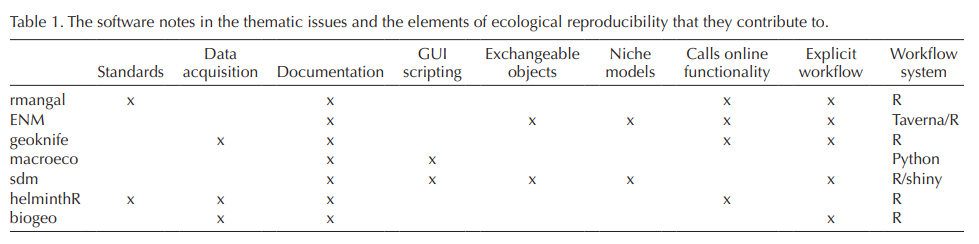
\includegraphics{images/Borregaard2016-01.png}}

\newpage
\newpage

\hypertarget{bibliographie}{%
\section*{Bibliographie}\label{bibliographie}}
\addcontentsline{toc}{section}{Bibliographie}

\hypertarget{refs}{}
\begin{CSLReferences}{0}{0}
\leavevmode\vadjust pre{\hypertarget{ref-baker2016reproducibility}{}}%
\CSLLeftMargin{1. }
\CSLRightInline{Baker M (2016) Reproducibility crisis. \emph{Nature}
533(26):353--66.}

\leavevmode\vadjust pre{\hypertarget{ref-barba2016hard}{}}%
\CSLLeftMargin{2. }
\CSLRightInline{Barba LA (2016) The hard road to reproducibility.
\emph{Science} 354(6308):142--142.}

\leavevmode\vadjust pre{\hypertarget{ref-borregaard2016towards}{}}%
\CSLLeftMargin{3. }
\CSLRightInline{Borregaard MK, Hart EM (2016) Towards a more
reproducible ecology. \emph{Ecography} 39:349--353.}

\leavevmode\vadjust pre{\hypertarget{ref-wang2016transparency}{}}%
\CSLLeftMargin{4. }
\CSLRightInline{Wang SV, et al. (2016) Transparency and reproducibility
of observational cohort studies using large healthcare databases.
\emph{Clinical Pharmacology \& Therapeutics} 99(3):325--332.}

\leavevmode\vadjust pre{\hypertarget{ref-haibe2020transparency}{}}%
\CSLLeftMargin{5. }
\CSLRightInline{Haibe-Kains B, et al. (2020) Transparency and
reproducibility in artificial intelligence. \emph{Nature}
586(7829):E14--E16.}

\end{CSLReferences}



% Bibliography
% \bibliography{pnas-sample}

\end{document}
